\documentclass[border=1pt,tikz,varwidth=\maxdimen]{standalone}

\usetikzlibrary{positioning,calc,arrows}

\usepackage{amsmath,mathtools}

\begin{document}
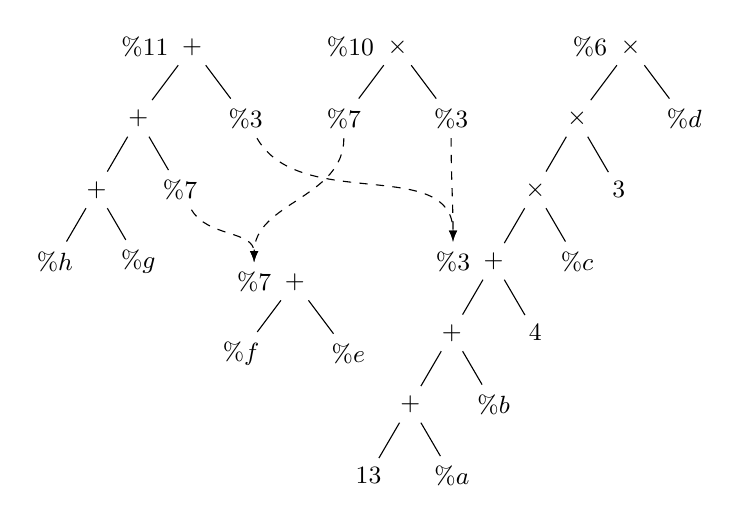
\begin{tikzpicture}[
  every node/.style={font=\small},
  level 1/.style={edge from parent,sibling distance=9ex,level distance=6ex},
  level 2/.style={edge from parent,sibling distance=7ex,level distance=6ex},
  dash-emph/.style={draw,dashed,-latex},
  ]

  \node (var11-tree-root) {\(+\)}
  child {
    node {\(+\)}
    child {
      node {\(+\)}
      child {
        node {\(\%h\)}
      }
      child {
        node {\(\%g\)}
      }
    }
    child {
      node (var11-tree-var7) {\(\%7\)}
    }
  }
  child {
    node (var11-tree-var3) {\(\%3\)}
  };
  \node [left=-0.5ex of var11-tree-root] (var11-text-node) {\(\%11\)};

  \node [right=6em of var11-tree-root] (var10-tree-root) {\(\times\)}
  child {
    node (var10-tree-var7) {\(\%7\)}
  }
  child {
    node (var10-tree-var3) {\(\%3\)}
  };
  \node [left=-0.5ex of var10-tree-root] (var10-text-node) {\(\%10\)};

  \node [below=5.25em of $(var11-tree-var3)!0.5!(var10-tree-var7)$] (var7-tree-root) {\(+\)}
  child {
    node {\(\%f\)}
  }
  child {
    node {\(\%e\)}
  };
  \node [left=-0.5ex of var7-tree-root] (var7-text-node) {\(\%7\)};

  \node [right=7em of var10-tree-root] (var6-tree-root) {\(\times\)}
  child {
    node {\(\times\)}
    child {
      node {\(\times\)}
      child {
        node (var3-tree-root) {\(+\)}
        child {
          node {\(+\)}
          child {
            node {\(+\)}
            child {
              node {\(13\)}
            }
            child {
              node {\(\%a\)}
            }
          }
          child {
            node {\(\%b\)}
          }
        }
        child {
          node {\(4\)}
        }
      }
      child {
        node {\(\%c\)}
      }
    }
    child {
      node {\(3\)}
    }
  }
  child {
    node {\(\%d\)}
  };
  \node [left=-0.5ex of var6-tree-root] (var6-text-node) {\(\%6\)};
  \node [left=-0.5ex of var3-tree-root] (var3-text-node) {\(\%3\)};

  \draw [dash-emph] (var11-tree-var7) to [out=300,in=90] (var7-text-node);
  \draw [dash-emph] (var10-tree-var7) to [out=270,in=90] (var7-text-node);

  \draw [dash-emph] (var11-tree-var3) to [out=300,in=90] (var3-text-node);
  \draw [dash-emph] (var10-tree-var3) to [out=270,in=90] (var3-text-node);

\end{tikzpicture}
\end{document}
